\section{Foundations of Agentic Visual Generation}
\label{sec:foundations}

\subsection{Visual Generation Foundations}
\label{sec:visual-foundations}

Visual generation in this survey covers the construction and editing of images, videos, three-dimensional scenes, parametric CAD models, scientific graphics, structured documents, interactive interfaces, and related visual products. Four foundations connect these operations to agentic control: the generator, the artifact representation, the conditioning inputs, and the execution interfaces. Together, they determine how an artifact is produced, what task-relevant information persists, what information an operation can use, and what actions the system can execute.

\begin{keytakeaway}[Four Foundations]
\begin{keypoints}
  \item \textbf{Generator:} produces or edits a visual artifact.
  \item \textbf{Representation:} preserves what can be inspected and modified later.
  \item \textbf{Conditioning:} supplies goals, references, constraints, and state.
  \item \textbf{Interface:} exposes callable operations, outputs, errors, and costs.
\end{keypoints}
\end{keytakeaway}

\subsubsection{Visual Generators}

In this survey, a visual generator is a model that maps a condition to a visual artifact or an editable visual representation. For a stochastic generator, the output $x$ can be written as a sample from a conditional distribution $p_{\phi}(x\mid c)$, where $c$ may contain text, images, spatial references, structured requirements, or information retained from an earlier operation. The main research question is therefore how a model represents $x$, how it parameterizes the conditional distribution, and which parts of $c$ can be used to control the result. The history of visual generators is best understood as a sequence of changes in representation and conditioning, with image and video models providing the main large-scale foundations and specialized systems adapting these foundations to structured outputs \cite{he2024llms,yang2025textimage,wang2025imageediting,yin2025spatiotemporal,wu2026visualgeneration}. Figures~\ref{fig:ch2-image-generators}--\ref{fig:ch2-multimodal} organize this development by output type, and each is discussed in the corresponding paragraph below.

\paragraph{Image foundation models.}
The first generation of neural image models focused on learning a data distribution from which new samples could be drawn. Variational autoencoders introduced an explicit latent-variable model with approximate inference, while generative adversarial networks learned a generator through a competition between a generator and a discriminator \cite{kingma2013autoencoding,goodfellow2014gan}. Normalizing flows added invertible transformations and tractable likelihood evaluation \cite{rezende2015variational,dinh2015nice}. In each case, training estimates a distribution over visual observations and inference samples from the learned distribution. The choice of latent variables, discriminator features, or invertible coordinates affects diversity, sharpness, likelihood estimation, and the ease with which a condition can be injected. These models established the separation between a representation space and a sampling procedure, and they made learned visual synthesis possible on data distributions that are difficult to specify with hand-written rules. Their interfaces were still mainly designed for unconditional sampling or a small set of manually designed conditions, so precise spatial control and reliable local editing were not yet central properties of the generator.

\begin{figure}[t]
  \centering
  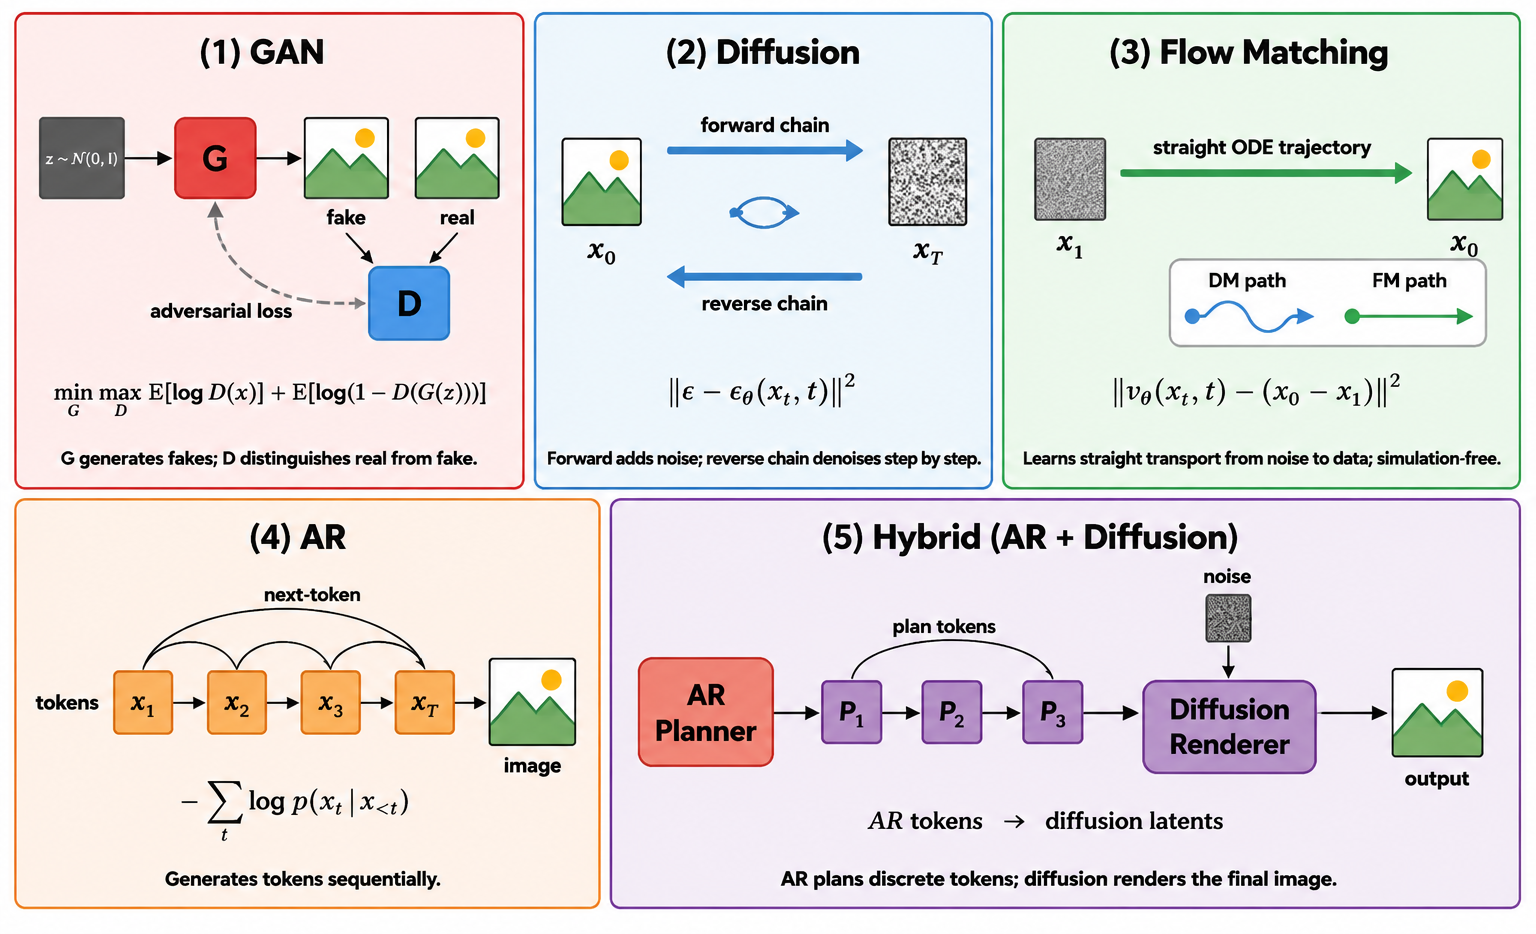
\includegraphics[width=\textwidth]{figures/ch2_image_generator.png}
  \caption{Representative image-generation paradigms. Generative adversarial networks, diffusion models, flow matching, autoregressive models, and hybrid autoregressive--diffusion systems differ in their latent representation, transport or decoding trajectory, and degree of iterative refinement.}
  \label{fig:ch2-image-generators}
\end{figure}

Autoregressive models then made the order of visual prediction explicit. PixelRNN predicted pixels sequentially, turning image synthesis into a conditional sequence model whose next prediction depends on the preceding context. VQ-VAE and VQGAN learned discrete visual representations that allowed an image to be treated as a sequence of tokens, and DALL-E used such a representation for large-scale text-conditioned generation \cite{oord2016pixelrnn,oord2017vqvae,esser2021vqgan,ramesh2021dalle}. The tokenizer became an important part of the generator: its codebook determines which visual details are retained, while the Transformer models dependencies among the resulting tokens. MaskGIT changed the decoding schedule by masking groups of tokens and filling them in parallel over several refinement steps, trading a strict left-to-right order for iterative global refinement \cite{chang2022maskgit}. Visual Autoregressive Modeling (VAR) organized prediction from coarse to fine scales, reducing the effective sequence length through next-scale prediction \cite{tian2024var}. LlamaGen and MAR revisit the same family at larger scale, with MAR modeling continuous token distributions together with a diffusion objective \cite{llamagen2024,mar2024}. This line of work therefore changes both the object being generated and the way generation proceeds: pixels become compact visual units, and a single pass becomes an ordered or iterative prediction process. The representation can be inspected, masked, reordered, or extended, which later supports token-level conditioning and editing.

Diffusion models formed a second major route for image foundation models. DDPM defined generation as the reversal of a gradual noising process: the model learns to remove noise at a sequence of noise levels, and sampling follows the learned reverse transitions from a noisy state to an image. Score-based formulations described the same family through the score of perturbed data distributions and connected discrete denoising to continuous stochastic differential equations \cite{ho2020ddpm,song2021scorebased}. Latent diffusion moved denoising into a compressed representation, separating perceptual compression from the generative process and making high-resolution synthesis more practical. Imagen demonstrated the effect of stronger language conditioning, while DiT replaced the convolutional denoiser with a Transformer operating on latent patches \cite{saharia2022imagen,rombach2022ldm,peebles2023dit}. Flow matching and rectified flow learn continuous transport paths between source and target distributions, and consistency models target one-step or few-step sampling by enforcing agreement among denoising trajectories \cite{lipman2022flowmatching,liu2022rectified,song2023consistency}. These formulations expose several controllable interfaces: the condition can enter at every denoising step, the latent representation can be edited before decoding, and the sampler can be selected according to a quality or latency requirement. They consequently provide the backends used by many later editing and agentic systems, while the number of sampling steps and the quality of the learned condition remain important practical variables. On the open-weights side, FLUX.1 scales rectified flow to a twelve-billion-parameter transformer and stands as the leading publicly available image generator of its generation \cite{blackforest2024flux}.

The most recent generation of image foundation models combines the two preceding routes within a single system. An autoregressive Transformer first predicts discrete image tokens conditioned on text and reference images, so the request is interpreted with the reasoning and instruction-following habits of language models; the hidden states of this backbone then serve as the condition for a diffusion model that renders the final image in continuous latent space, inheriting the rendering quality of denoising. BLIP3o-NEXT identifies this composition as the current default for open-weight native image generators \cite{blip3o2025next}. HunyuanImage 3.0 scales the recipe to an 80-billion-parameter mixture-of-experts language model with chain-of-thought supervision \cite{hunyuanimage3_2025}, Qwen-Image pairs a vision-language condition encoder with a multimodal diffusion transformer for paragraph-level text rendering \cite{qwenimage2025}, and FLUX.2 combines a 32-billion-parameter rectified-flow transformer with a 24-billion-parameter vision-language encoder \cite{flux2_2025}. Reinforcement-learning post-training is applied on top of this composition, transferring the policy-optimization infrastructure of large language models to image generation and improving text rendering and instruction following beyond supervised finetuning \cite{qwenimage2rl_2026}. In this setting, text, reference images, and spatial signals such as masks, edges, and depth enter through a single multimodal conversation, and operations that previously required separate editing pipelines reduce to a prompt. Figure~\ref{fig:ch2-image-generators} contrasts the five paradigms by latent representation, transport trajectory, and degree of iterative refinement.

\paragraph{Video foundation models.}
Video generators extend image generation with a temporal representation: an output is a sequence whose frames must remain individually plausible while preserving motion, identity, and scene continuity, so the generator models correlations across space and time under conditions that may specify an initial frame, a motion pattern, a camera change, or a textual event. Early attempts used video GANs, recurrent predictors, and 3D convolutions, but they produced only seconds-long, low-resolution clips because adversarial objectives remained difficult to stabilize over high-dimensional spatiotemporal data \cite{tulyakov2018mocogan,clark2019dvdgan}.

The field shifted decisively in 2022 along two parallel routes. The autoregressive route modeled video as ordered discrete tokens: CogVideo scaled this idea to a nine-billion-parameter transformer and became the first large-scale open-source pretrained text-to-video system, while Phenaki coupled a causal video tokenizer with a transformer to generate minute-level sequences from chained prompts \cite{hong2022cogvideo,villegas2022phenaki}. The diffusion route transplanted image denoisers to spatiotemporal data: Video Diffusion Models established the core formulation with factorized noise trained jointly on images and videos \cite{ho2022videodiffusion}, Make-A-Video showed that a text-to-image prior can supply appearance while unlabeled video supplies motion, avoiding paired text-video supervision altogether \cite{singer2022makeavideo}, and Imagen Video composed seven cascaded diffusion stages for progressive refinement \cite{ho2022imagenvideo}.

Work from 2023 onward consolidated around latent diffusion with explicit temporal modules. ModelScopeT2V combined a text encoder, VQGAN, and a denoising UNet with spatiotemporal blocks into a widely replicated design \cite{modelscope2023}. Instead of learning appearance and motion jointly, systems reused frozen text-to-image backbones and inserted lightweight temporal layers: AnimateDiff added a plug-and-play motion module, Stable Video Diffusion specialized a latent backbone for image-to-video synthesis, and Emu Video factored text-to-video into text-to-image followed by image-to-video \cite{guo2023animatediff,blattmann2024svd,he2022emuvideofactorizing}. This strategy reduced training cost substantially while inheriting the prompt-following behavior and visual diversity of strong image priors.

A second inflection arrived with OpenAI's Sora, which replaced convolutional denoisers with a diffusion transformer operating on spacetime patches at native resolution and duration, making a single scalable architecture handle still images, short clips, and extended sequences interchangeably \cite{brooks2024sora}. Foundation-scale systems followed in quick succession: Movie Gen paired a thirty-billion-parameter video model with a dedicated thirteen-billion-parameter audio model for joint generation, CogVideoX unified spatial and temporal modeling inside a single 3D full-attention block as the open-source successor to CogVideo, and HunyuanVideo and Wan advanced open-source alternatives with larger corpora, temporal compression, and efficient inference \cite{girdhar2024moviegen,yang2024cogvideox,kong2024hunyuanvideo,wan2025}. Their interfaces now span text-to-video, image-to-video, video extension, camera trajectories, and reference-conditioned editing, shifting the focus from rendering isolated frames toward modeling a temporally persistent visual state in which objects survive, cameras move, and actions unfold across many seconds. Joint audio-visual generation marks the current frontier: Veo 3 produces synchronized dialogue, effects, and ambient sound alongside frames by processing visual spacetime patches and temporal audio channels within one diffusion pass \cite{deepmind2025veo3}, and recent releases across proprietary and open-source families continue to push duration, resolution, and prompt adherence upward. Figure~\ref{fig:ch2-video-generators} traces this progression from early spatiotemporal extensions to foundation-scale audio-visual systems.

\begin{figure}[t]
  \centering
  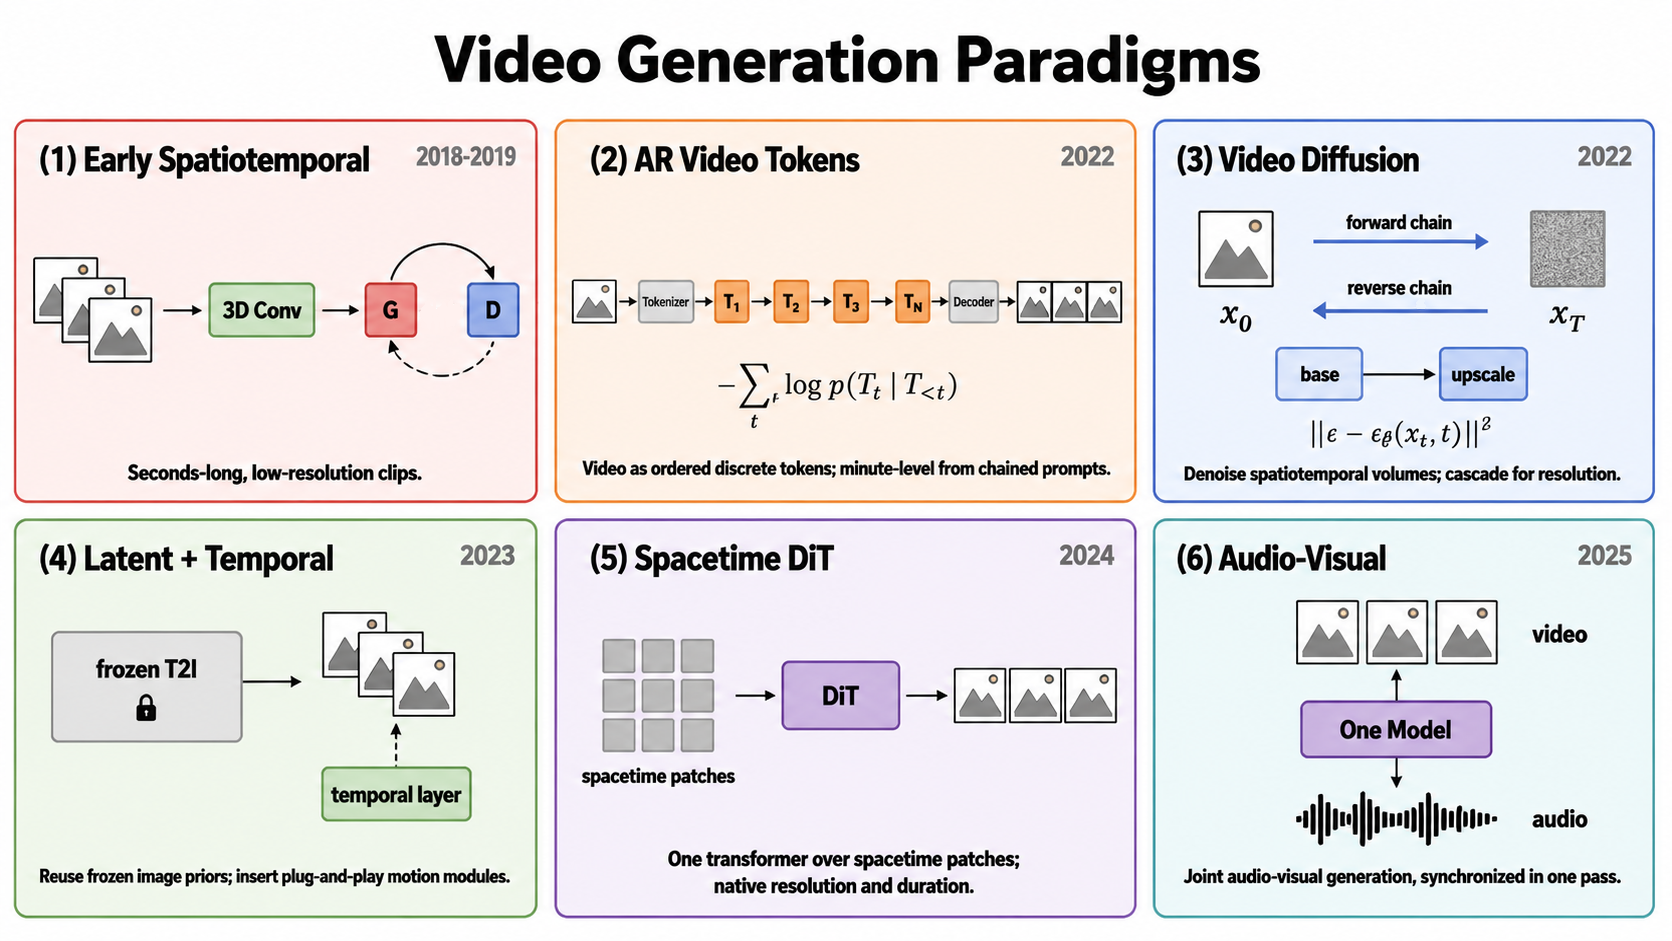
\includegraphics[width=\textwidth]{figures/ch2_video_generator.png}
  \caption{Representative video-generation paradigms. Early spatiotemporal extensions, autoregressive token models, latent diffusion with temporal modules, and foundation-scale diffusion transformers differ in how they factor space and time, in their conditioning surface (initial frames, motion patterns, camera trajectories), and in whether audio is generated jointly with frames.}
  \label{fig:ch2-video-generators}
\end{figure}

\paragraph{3D and world foundation models.}
Three-dimensional generators use representations such as voxels, point clouds, meshes, neural fields, or Gaussian primitives, which differ in how they encode geometry, appearance, topology, and view-dependent effects, and determine whether a generated object can be rendered, measured, or edited after synthesis. NeRF first showed that a continuous neural field maps spatial locations and viewing directions to density and color, making a scene renderable from new viewpoints \cite{mildenhall2020nerf}. DreamFusion then used a pretrained two-dimensional diffusion model as a prior and optimized a three-dimensional representation through repeated rendering, establishing the influential route to text-to-3D when large paired 3D datasets were scarce, at the cost of slow per-instance optimization and sensitivity to multi-view consistency \cite{poole2022dreamfusion}.

The following stage emphasizes faster reconstruction and more explicit scene representations. 3D Gaussian Splatting represents a scene with oriented, colored Gaussian primitives for real-time radiance-field rendering \cite{kerbl2023gaussiansplatting}, while LRM, TripoSR, VFusion3D, and Hunyuan3D replace per-instance optimization with learned feed-forward mappings from image or multi-view-diffusion evidence to 3D assets \cite{lrm2023,triposr2024,vfusion3d2024,hunyuan3d2024}. TRELLIS extends this line toward editable structure: its structured latents decode a single generated object into radiance fields, Gaussians, or meshes, support tuning-free local editing, and scale to rectified-flow transformers with up to two billion parameters trained on 500K objects \cite{xiang2024trellis}. Together, these systems make 3D generation suitable for repeated calls inside larger workflows, although geometric completeness and cross-view agreement remain central quality dimensions.

The current frontier extends from individual assets to scenes, dynamic environments, and interactive worlds along three lines of work. Video-trained world models generate action-controllable environments: Genie 2 turned a prompt image into keyboard-playable scenes persisting for tens of seconds, and Genie 3 sustains real-time navigation at 720p and 24~fps over several minutes \cite{parkerholder2024genie2,parkerholder2025genie3}. Physics-aware world foundation models target embodied use at scale: Cosmos couples large-scale pretraining with future-state video prediction for robots and autonomous vehicles and releases early checkpoints under an open license \cite{nvidia2025cosmos}. Diffusion-based neural game engines learn interactivity end to end: GameNGen simulates DOOM interactively above 20 frames per second on a single TPU by conditioning next-frame generation on recorded actions, and the open-source Oasis demonstrates real-time Minecraft-style play \cite{valevski2024gamengen,decart2024oasis}.

A world-oriented generator must preserve spatial relations across objects, support changes over time, and define how an observation, an action, and a subsequent visual state are related, properties that distinguish a world model from a generator that produces a single plausible object. Figure~\ref{fig:ch2-3d} contrasts these routes by representation explicitness, reconstruction cost, and whether the output couples observation, action, and subsequent visual state.

\begin{figure}[t]
  \centering
  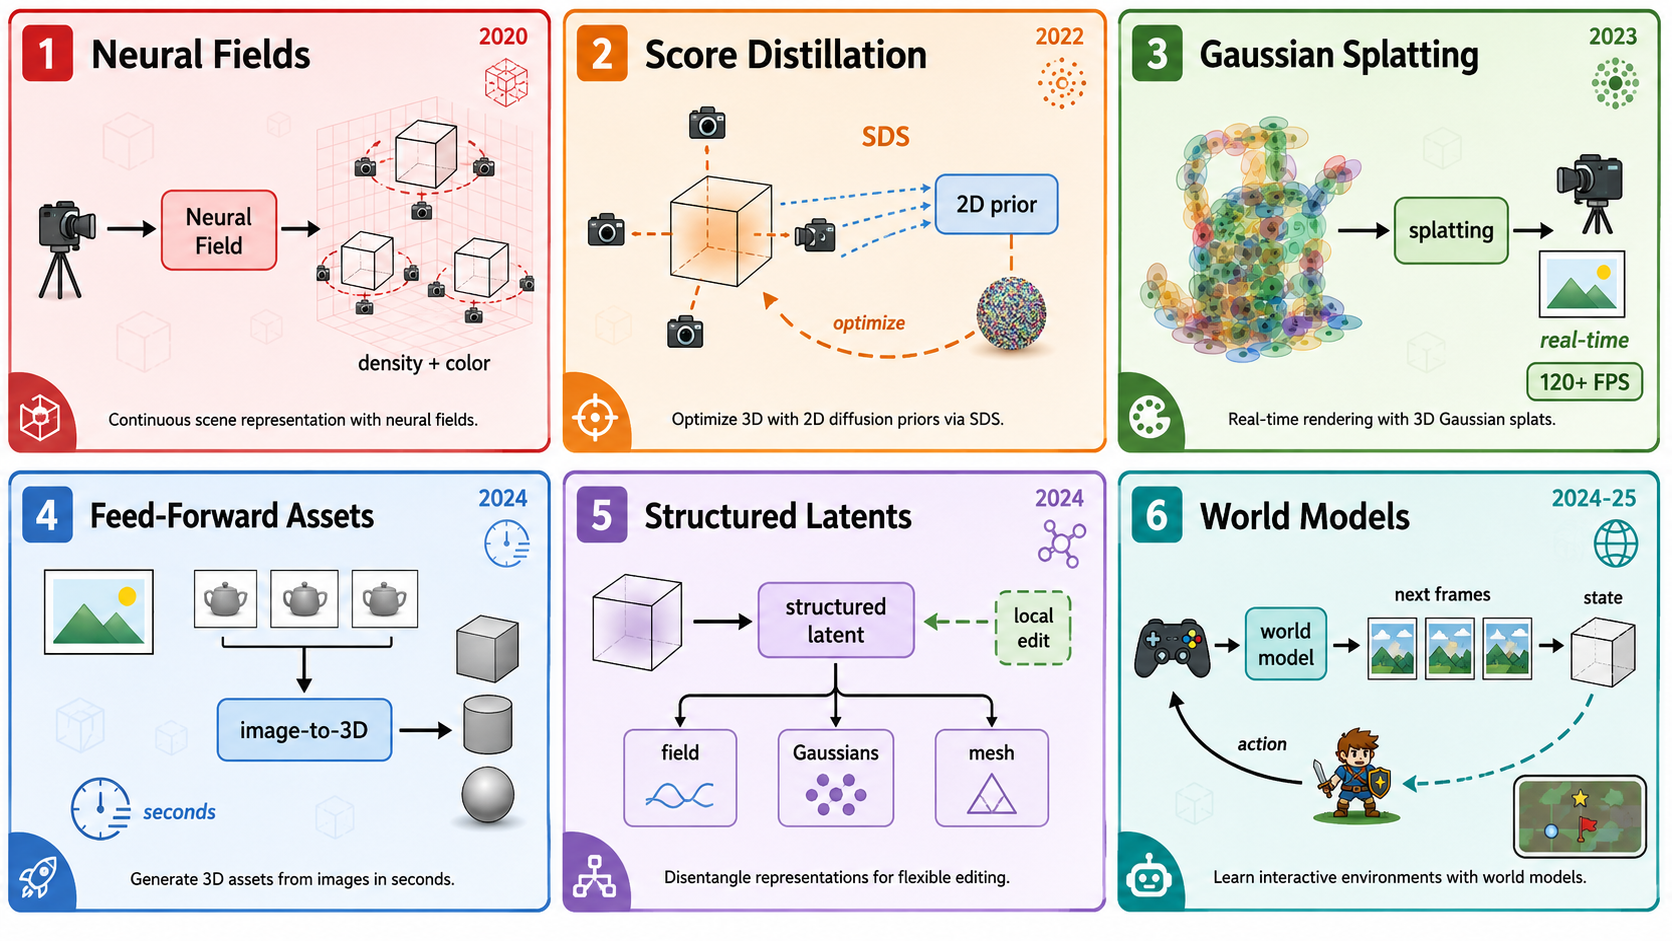
\includegraphics[width=\textwidth]{figures/ch2_3d.png}
  \caption{Representative 3D and world generation paradigms. Neural fields, feed-forward asset reconstruction, editable structured latents, and action-controllable world models differ in how explicitly geometry and appearance are represented, in per-instance optimization versus feed-forward reconstruction, and in whether the generated environment couples observation, action, and subsequent visual state.}
  \label{fig:ch2-3d}
\end{figure}

\paragraph{Structured and executable visual generators.}
Some visual tasks require a representation that remains editable or executable after rendering. In these tasks, the generator outputs a layout tree, a visualization specification, a construction sequence, or source code alongside the rendered view, so that the produced artifact can be inspected, modified, and re-rendered rather than delivered only as a final appearance. This distinguishes the generators in this paragraph from those in the preceding ones: an image or video model terminates at rendered pixels, whereas a structured generator preserves the internal construction that produced those pixels, which is what allows a later operation to target a specific component, parameter, or code block. The development of this family (covering layout, chart, document, CAD, and UI generation) progressed through four stages, drawing on research communities that worked largely in parallel before converging in the LLM era.

Early systems came from the human--computer interaction community and relied on templates, visual grammars, and component libraries, with hand-designed rules guaranteeing structural validity at the cost of coverage bounded by the available templates and production rules \cite{landay2001sketching}. The neural stage arrived with sequence-to-sequence translation from the NLP community: Data2Vis mapped data specifications to Vega-Lite visualization programs with an attention-based LSTM \cite{dibia2018data2vis}, and pix2code generated platform-specific interface code directly from a GUI screenshot with over 77\% accuracy across iOS, Android, and web targets \cite{beltramelli2017pix2code}, establishing that structured output can be learned end to end rather than authored.

Work from 2021 onward turned to construction sequences, replacing a final artifact with a program whose rendering is repeatable and editable. DeepCAD trained a Transformer-based autoencoder on 178{,}238 Onshape models to generate sketch-and-extrude sequences that preserve construction history rather than only a final mesh \cite{wu2021deepcad}; SkexGen disentangled topology, geometry, and extrusion into separate codebooks for finer control \cite{xu2022skexgen}; and LayoutDM handled controllable layout generation across multiple tasks with modality-wise discrete diffusion \cite{inoue2023layoutdm}. Because the generated object is a structured description rather than a rendered view, a later operation can inspect the construction history, modify a step, and re-render, associating a visible defect with a source-level element.

The current stage connects general-purpose language and multimodal models to these structured representations, and in doing so merges the previously separate communities. A model can produce HTML/CSS/JavaScript, a chart specification, or a CAD program and hand the result to a renderer, parser, or execution environment: LIDA generates grammar-agnostic visualizations from natural-language summaries of data \cite{dibia2023lida}. Benchmarking efforts such as Design2Code evaluate multimodal models on converting webpage screenshots into code, and find that models mostly lag in recalling visual elements and generating correct layouts \cite{si2024design2code}; Sketch2Code extends this line to low-fidelity hand-drawn sketches and further shows that even the strongest models struggle to interpret sketches and to formulate clarifying questions in multi-turn interaction \cite{li2024sketch2code}. Across structured domains, the long-term trend is from rendering a finished appearance to generating an editable or executable object whose consequences can be observed, with each community contributing a distinct structural prior that LLM-era systems now inherit together. Figure~\ref{fig:ch2-structure} depicts the four stages and the structural priors each contributed.

\begin{figure}[t]
  \centering
  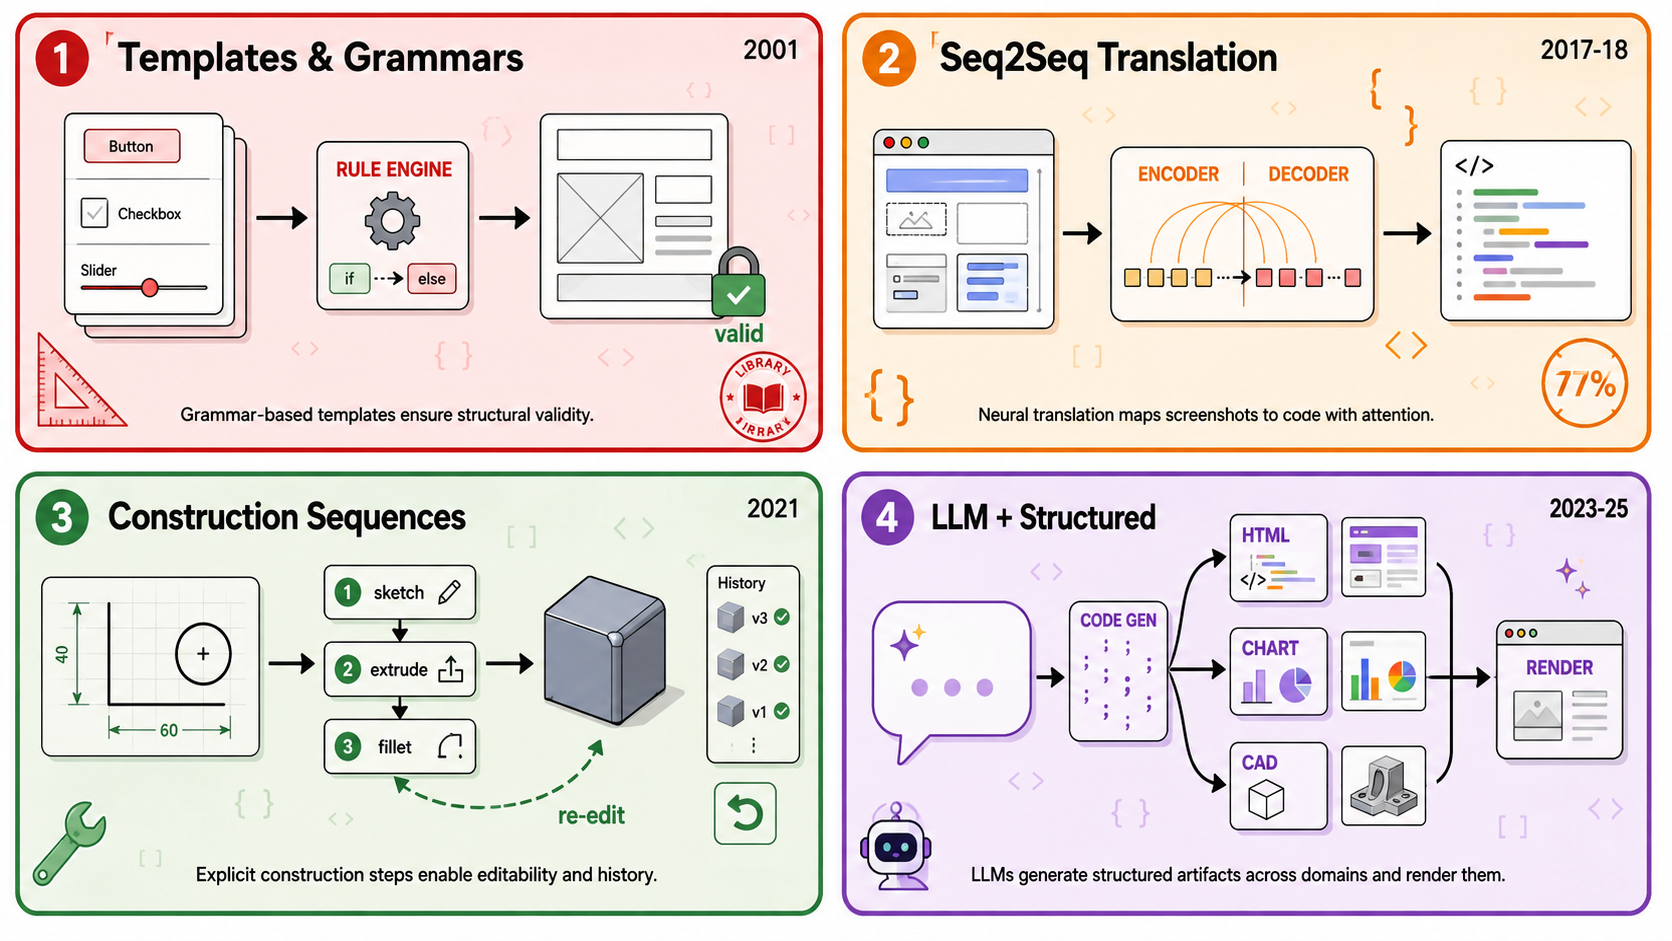
\includegraphics[width=\textwidth]{figures/ch2_structure.png}
  \caption{Representative structured and executable generation paradigms. Template- and grammar-based systems, sequence-to-sequence translation, construction-sequence models, and LLM-based structured generation differ in how the editable object is produced, which structural prior it inherits (grammars, source data, construction history, code), and how a later operation can target components, parameters, or code blocks.}
  \label{fig:ch2-structure}
\end{figure}

\paragraph{Unified multimodal visual generation models.}
The development of visual generators also includes a cross-modal route that unifies visual understanding and generation. Unlike the preceding paragraphs, which are organized by the type of visual output, this line is organized by how understanding and generation are coupled within a single model. Its first stage keeps modality-specific encoders and decoders around a shared language or Transformer representation: text is encoded into a condition, the visual generator produces an artifact, and a separate vision encoder interprets the result. The interfaces are clear, but information must be translated whenever the system moves between understanding and generation. Mixed-token models reduce this separation by placing text and visual content in one sequence: Chameleon and Emu3 model mixed visual--textual sequences, and Show-o combines autoregressive prediction with discrete diffusion so that the same backbone can interpret context and produce visual content \cite{chameleon2024,emu32024,showo2024}. A new visual prediction can now be conditioned on an earlier image, a textual explanation, and preceding visual tokens without constructing a task-specific interface for each transition, which broadens the information a generator can consume and lets generation draw on visual context, intermediate representations, and language-level reasoning.

The next stage introduces specialized tokenizers or encoding paths within a unified system, because understanding favors features that preserve semantic distinctions while generation requires representations that retain appearance and permit high-quality decoding. Janus separates visual encoding paths for understanding and generation while retaining a unified multimodal interface \cite{janus2024}. This organization supports image-conditioned generation, visual question answering followed by editing, and interleaved multimodal output, with trade-offs among understanding accuracy, generation quality, tokenization choices, and inference cost. The pathway choice also determines which intermediate representation can be passed to a later operation: a shared sequence can retain multimodal context, while a specialized generative latent can support efficient rendering.

The current frontier carries this route into production-scale systems. GPT-4o generates images natively inside the language model: an autoregressive decoder interleaves text tokens with continuous image latents that a diffusion head decodes, so the same conversational context drives both dialogue and synthesis, yielding accurate in-image text rendering, detailed multi-object instruction following, and edits that build on previous turns \cite{openai2025gpt4oimage}. Gemini 2.5 Flash Image extends the same interface toward editing: it pairs multi-image fusion with character and style consistency across generated sequences and led the LMArena image-editing leaderboard at release, turning reference-preserving, conversation-driven editing into a first-class capability rather than a mask-driven pipeline \cite{deepmind2025flashimage}. Across these systems the condition space converges on multimodal conversation itself, where reference images, instructions, and dialogue history jointly determine what is generated. Unified multimodal modeling is a foundation-model direction: it determines what a single model can consume and produce. Figure~\ref{fig:ch2-multimodal} contrasts the four coupling stages.

\begin{figure}[t]
  \centering
  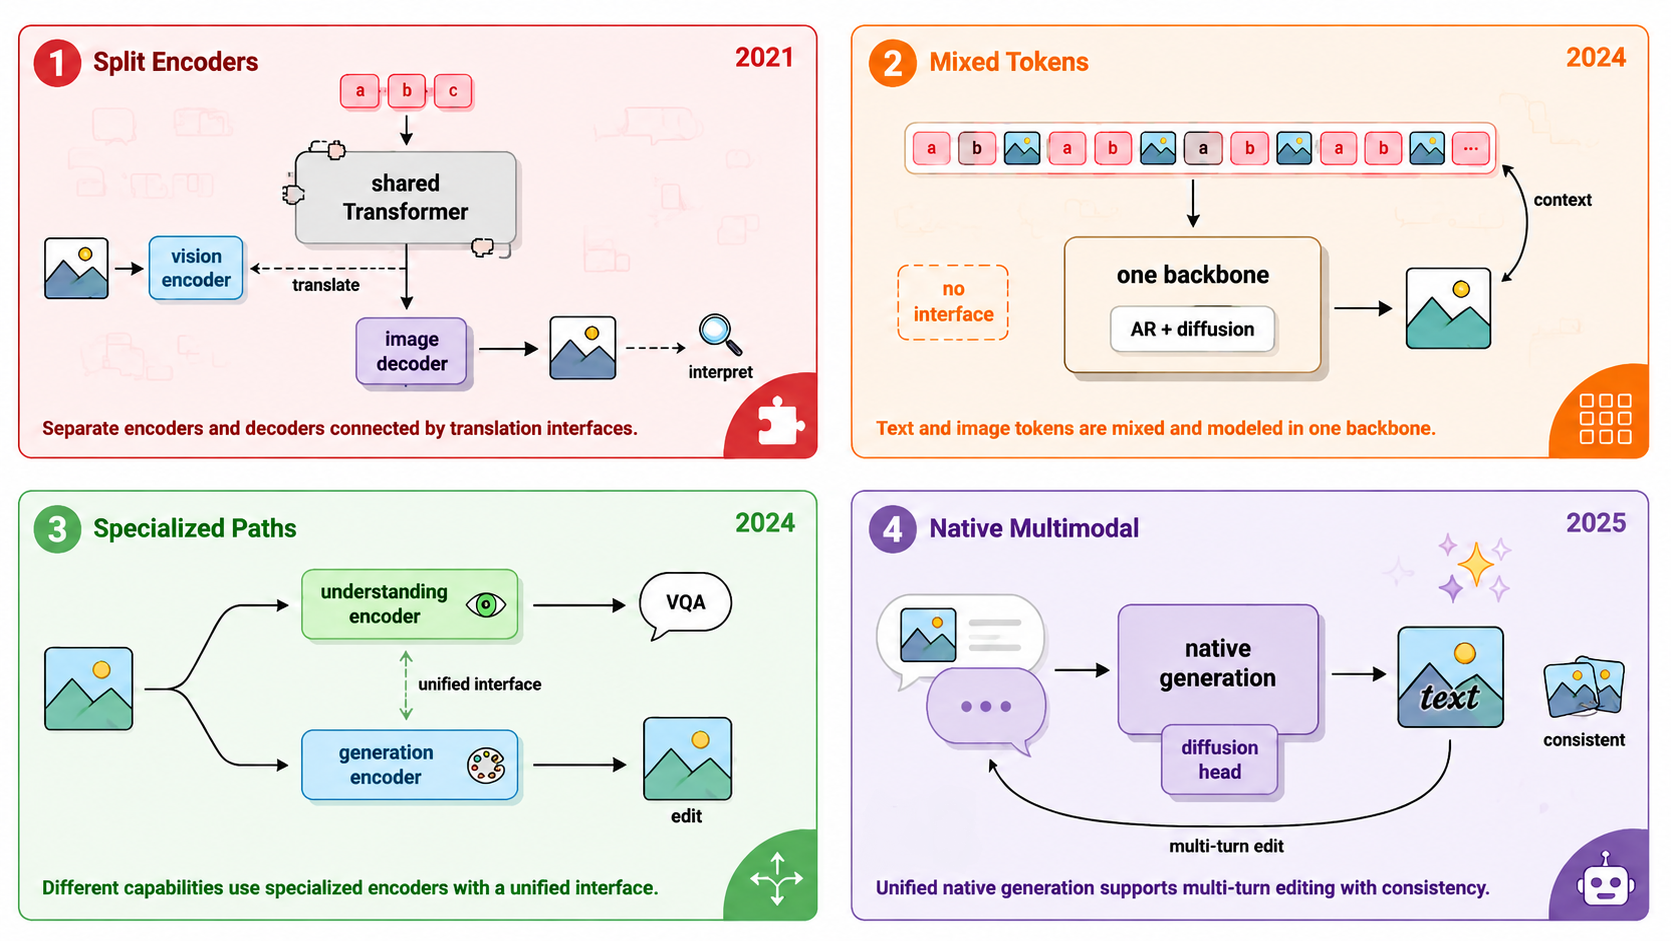
\includegraphics[width=\textwidth]{figures/ch2_multimodal.png}
  \caption{Representative unified multimodal generation paradigms. Split encoders around a shared Transformer, mixed-token sequences, specialized encoding paths, and native multimodal generation differ in how understanding and generation are coupled, which intermediate representations are shared between them, and what conditions the generator can consume in a single conversation.}
  \label{fig:ch2-multimodal}
\end{figure}

\begin{keytakeaway}[Visual Generators: What Matters for Control]
\begin{keypoints}
  \item \textbf{Two properties decide agentic usability:} which conditions a generator can consume, and which representation it exposes for later operations.
  \item \textbf{Image generators:} the controllable surface spans several levels: token sequences expose inspectable, reorderable units for token-level conditioning and editing; continuous-latent generators accept conditions at every step and expose editable latents; masks, instructions.
  \item \textbf{Video generators:} the unit of control is a temporally persistent visual state rather than isolated frames (identity, motion, and scene continuity must survive across the sequence), and conditions extend to initial frames, motion patterns, camera trajectories, and reference-based editing; joint audio--visual generation marks the current frontier.
  \item \textbf{3D and world generators:} the output representation determines whether an asset can be rendered, measured, or edited after synthesis; world models further couple observation, action, and subsequent visual state, making the generator itself an action-controllable environment.
  \item \textbf{Structured generators:} construction history survives rendering, so a later operation can target a component, parameter, or code block.
  \item \textbf{Unified multimodal models:} understanding and generation are unified in one model; the condition space converges on multimodal conversation itself.
\end{keypoints}
\end{keytakeaway}


\subsubsection{Visual Artifacts and Task Evidence}

A visual artifact is the object that a system creates, edits, or delivers. Common forms include rendered images and videos, structured scene or geometric representations, data-grounded graphics, documents, interactive interfaces, and related artifacts. Depending on its representation, an artifact may contain rendered appearance together with temporal relations, geometry, parameters, source data, hierarchy, or interaction state. These representations can preserve task-relevant properties across operations \cite{yin2025spatiotemporal,mildenhall2020nerf,wu2021deepcad,dibia2018data2vis,beltramelli2017pix2code}.

The same visual result can be carried by different representations. A poster, for example, may exist as a raster image, as a layered graphics file, or as a parameterized template: the rendered appearance is identical, yet a raster image supports only appearance-level edits, the layered file allows object-level changes, and the template turns a single parameter change into a global update. An artifact is therefore characterized by the representation in which it persists between operations, not only by its rendered appearance.

The artifact representation, together with the task requirements, helps determine what constitutes a valid result. Video tasks may require temporal preservation of identities, events, motion, camera changes, and other sequence-level properties. Three-dimensional and CAD representations can expose geometry, topology, parameters, and construction constraints. Data-driven graphics may retain links to source data, structured documents may retain layout or hierarchy, and interfaces may retain executable behavior. Other visual products impose their own representation-specific requirements and sources of evidence.

Across these forms, validity requirements group into a few recurring kinds. One kind asks whether the artifact faithfully realizes the condition: whether an edited image follows the instruction while preserving the rest, or whether a generated page matches the request. A second kind asks whether the artifact is internally consistent: whether video frames cohere into a continuous sequence, whether a mesh closes into a manifold, or whether cross-references inside a document resolve. A third kind checks the artifact against external references: whether a chart's plotted values match the underlying table, whether a generated model respects the specified dimensions, or whether an interactive page behaves correctly when exercised. Each kind calls on different evidence.

Correctness therefore depends on evidence matched to the representation and the task, such as temporal checks, geometric or constraint checks, data consistency, layout inspection, or functional execution. A representation also sets the upper bound on what can be verified: pixel-only artifacts admit appearance comparison, while representations that retain construction, structure, or code admit structural and functional checks as well. The representation and the available operations together determine which properties can be inspected, preserved, or modified later.

\begin{keytakeaway}[Artifact Representation and Verifiability]
\begin{keypoints}
  \item \textbf{Representation is not neutral:} the same visual result carried by different representations supports different later operations.
  \item \textbf{Three recurring validity kinds:} faithfulness to the condition, internal consistency, and agreement with external references; each kind calls on different evidence.
  \item \textbf{Representation bounds verification:} pixel-only artifacts admit appearance comparison; representations retaining construction, structure, or code admit structural and functional checks as well.
\end{keypoints}
\end{keytakeaway}

\subsubsection{Conditioning Inputs}

A conditioning input is information supplied before a particular generation or editing operation. It helps specify what that operation should create, preserve, or change. The main forms are textual instructions, visual or spatial references, and structured task information. Text provides semantic intent and requested content; visual or spatial references provide appearance, identity, location, or layout cues; structured information provides explicit data values, geometric constraints, programmatic specifications, or other task requirements \cite{yang2025textimage,wang2025imageediting,yin2025spatiotemporal}.

The three forms differ in what they fix and what they leave open. Text may state a complete request or a single attribute to change, and the same words can carry an intent to realize, a style to imitate, or a constraint to respect. A visual reference likewise plays different roles: the same image may serve as content to preserve, an identity to transfer, a composition to follow, or the canvas of an edit. Structured information is the most explicit form: a data table, a schema, a layout tree, or a program pins down values and relations that text describes only loosely. A condition is thus a partial specification of the task.

The role of a condition depends on the operation that receives it. An initial operation may use a user request and reference material, while a later operation may use the current artifact, a selected region, an intermediate specification, or a verified state. These inputs make some task variables explicit while leaving other requirements to be inferred, clarified, or checked after execution. They also affect the granularity of control, which follows from both the form of the condition and the representation of the artifact: a text prompt acts on the whole output, a mask or a box restricts the change to a region, a reference to an object addresses one element of a structured scene, and a single parameter touches one construction step; the latter granularities exist only when the artifact representation retains the corresponding structure.

Over a sequence of operations, the composition of conditions shifts. Early operations are driven mainly by user-supplied conditions; as the artifact takes shape, later operations increasingly consume what the system itself has produced, and the original request turns from a primary driver into a background constraint on everything that follows. Several conditions also routinely enter one operation together, each constraining a different dimension: an instruction states what to change, a region states where, a reference image states how the result should look, and structured values state what must remain exact.

\begin{keytakeaway}[Conditioning Inputs]
\begin{keypoints}
  \item \textbf{Three forms with different explicitness:} text states intent and requested content; visual and spatial references carry appearance, identity, and layout cues; structured information pins down values and relations that text describes only loosely.
  \item \textbf{Conditions are partial specifications:} each form fixes part of the task and leaves the remainder to the model, later operations, or verification.
  \item \textbf{Granularity is joint:} control granularity follows from the condition form and the artifact representation together; fine granularities exist only when the representation retains the corresponding structure.
  \item \textbf{Drivers shift over a trajectory:} later operations increasingly consume system-produced state, and the original request becomes a background constraint.
  \item \textbf{Conditions compose:} one operation routinely receives several conditions, each constraining a different dimension.
\end{keypoints}
\end{keytakeaway}


\subsubsection{Execution Interfaces}

An execution interface is the callable boundary through which a controller invokes an operation on an artifact or task environment, or obtains task-relevant execution evidence. It defines the callable operations, accepted inputs, returned outputs, and execution status or error information made available to the controller. For a structured artifact, an operation may alter a representation or render it; for an interactive interface or other executable artifact, it may run code, tests, or interaction steps. Interfaces differ in operation granularity and feedback channels. They connect a controller decision to an artifact or environment update, or to task-relevant execution evidence \cite{he2024llms,yin2025spatiotemporal}. A controller never touches the artifact directly: every change it makes passes through such a boundary, and every observation it receives is whatever the boundary returns.

The operations an interface can offer are bounded by the representation beneath it. Pixel-level artifacts admit regeneration and appearance edits; layered or structured artifacts admit object- and parameter-level selection and modification; executable artifacts admit running, testing, and debugging. What the interface returns is subject to the same bound. Beyond the updated artifact, an interface can report status and diagnostics (which step failed, or which constraint was violated), and this localization is what allows a later operation to target the cause rather than the symptom.

Conditions specify the information and requirements for an operation, whereas execution interfaces specify how that operation can be carried out. The available operations and their granularity determine whether a controller can make a global change, edit a local region or object, modify a parameter, call a verifier, or invoke a recovery operation. Their outputs determine what the controller can observe after execution, including a new artifact, a rendering, a structured result, an error, or a test outcome. Together, these properties define the action space and the execution evidence available at each point in a visual creation process.

\begin{keytakeaway}[Execution Interfaces]
\begin{keypoints}
  \item \textbf{Single channel:} every controller change and every observation passes through the callable boundary.
  \item \textbf{Bounded by representation:} available operations and returned outputs are determined by what the artifact representation retains.
  \item \textbf{Diagnostics:} status and error information let a later operation target the cause rather than the symptom.
  \item \textbf{Action space:} operations and their granularity determine what can be changed; outputs determine what can be observed.
\end{keypoints}
\end{keytakeaway}




\subsection{Definition of Agentic Visual Generation}
\label{sec:agentic-visual-generation}

\subsubsection{Behavioral Definition}

Agentic visual generation is identified by how a system controls a visual creation trajectory. The controller faces recurring decision points: which operation or tool to invoke, which repair target to address, whether to continue or stop, and related decisions that range from clarification and planning to verification, revision, recovery, and termination \cite{xie2024large,durante2024agentai,jiang2024rationality,schneider2025generative}. The creation process operates through a closed loop when runtime observations of the evolving artifact, its task environment, and the interaction history change what the system selects at these points.

The formal definition is:

\begin{quote}
\emph{Agentic visual generation (AVG) is goal-driven visual creation organized as a closed loop over a multi-step trajectory. At the decision points exposed to the controller (which operation or tool to invoke, which repair target to address, whether to continue or stop, and related decisions), the system selects among available alternatives based on runtime observations drawn from accessible, task-relevant state spanning the evolving visual artifact, its task environment, and the interaction history, which is in turn updated by intermediate artifacts, execution outcomes, external information, user feedback, and other task-relevant sources.}
\end{quote}

The defining behavioral criterion is therefore a demonstrable observation--action dependency: different runtime observations lead to different selected actions. The next subsubsection formalizes this criterion as a condition on the action distribution and states the operational test used throughout the survey.

The definition is applied by examining a system's creation trajectory. The task concerns the creation, editing, or construction of a visual artifact or an editable visual environment. An identifiable decision process faces the decision points above and retains task-relevant state in a form accessible at later decision points. This state is updated by intermediate artifacts, execution outcomes, external information, user feedback, and other task-relevant sources, and observations drawn from it are shown to change a later action selection or parameterization. The decision process may be implemented by a single model, a learned policy, a search procedure, or a hierarchy of specialized agents; the same trajectory-level criterion applies across these implementations.

\subsubsection{Formalization of Closed-Loop Visual Creation}

The four foundations above specify what can be produced, what representation is retained, what information is supplied to an operation, and how that operation is invoked. We abstract a visual-creation trajectory using these same elements. Let $g$ denote the task goal and its requirements, $x_t$ the current artifact representation, $s_t$ the relevant state of the task environment, $h_t$ the accessible interaction history up to step $t$, and $\mathcal{I}_t$ the execution interfaces available at step $t$. The triple $(x_t,s_t,h_t)$ instantiates the accessible, task-relevant state of the definition: the evolving visual artifact, its task environment, and the interaction history. We write $z_t=(x_t,s_t,h_t)$ for this joint accessible state. The artifact representation $x_t$ may be a rendered image or video, a structured scene or geometric model, a document or layout, executable interface code, or another representation appropriate to the task. The environment state $s_t$ includes information needed to continue execution, such as application state, source data, files, or execution results. The history $h_t$ records prior actions, observations, outcomes, and user interactions. The formulation instantiates a POMDP whose information state is $z_t$: because $h_t$ carries the full interaction history, the state needed for the next decision is fully contained in $z_t$, and the policy conditions only on $g$, on quantities derived from $z_t$, and on $\mathcal{I}_t$.

Each step consists of a read, a decision, and a write. The read produces the runtime observation available to the controller:
\begin{equation}
  o_t = \mathsf{O}(g,x_t,s_t,h_t).
\end{equation}
The dependence on $g$ expresses that reads from the state are task-relevant. The observation $o_t$ may contain a visual inspection, a structured property, an execution result, a constraint check, external information, or user feedback, depending on the artifact and task. The decision, conditioned on the observation, selects among the available alternatives and parameterizes the selected action. When the action invokes an execution interface, it can be written as $a_t=(i_t,c_t)$, where $i_t\in\mathcal{I}_t$ is the selected interface and $c_t$ is the condition and operation input supplied to it. The action can also be a control decision such as revising the plan, recovering from an error, or stopping:
\begin{equation}
  a_t \sim \pi_{\theta}\!\left(\cdot \mid g,o_t,h_t,\mathcal{I}_t\right).
\end{equation}
The support of $\pi_{\theta}$ corresponds to the available alternatives: the callable interfaces in $\mathcal{I}_t$, their parameterizations, and the control decisions. Because $a_t$ includes both the interface and its condition, the observation--action dependency covers action selection and parameterization alike.

The write applies the selected action to the state through the execution interfaces. The interface set $\mathcal{I}_t$ is the callable boundary described above: it determines which operations can be invoked, which conditions they accept, and which artifact updates, execution outcomes, or status information they return. When $a_t=(i_t,c_t)$ invokes a stochastic generator, its output can be written as $x_{t+1}\sim p_{\phi}(\cdot\mid c_t)$ for a new artifact. For editing and structured construction, the same interface updates an existing representation. Both cases are represented by a Markov-kernel transition
\begin{equation}
  (x_{t+1},\,s_{t+1},\,h_{t+1},\,\mathcal{I}_{t+1})
  \;\sim\;
  \mathsf{U}\!\left(\cdot\,\middle|\,g,\,x_t,\,s_t,\,h_t,\,a_t;\,\mathcal{I}_t\right),
\end{equation}
in which the artifact channel $p_{\phi}(\cdot\mid c_t)$ supplies the stochastic component, and the remaining bookkeeping, including the update of $s_t$ and $h_t$ and the recording of any evidence returned by the interface, is deterministic given the drawn artifact. The kernel additionally returns the next interface set $\mathcal{I}_{t+1}$, allowing interfaces to become available, fail, or be retired as the artifact evolves; when the interface set is static this component is the identity. The process terminates when the controller selects a stopping decision; stopping acts as an absorbing transition after which no further observations are drawn, and the criterion below is evaluated over the steps before termination.

The write feeds the next read: the updated artifact and environment produce new runtime observations, which are available to the next decision. This is the write side of the definition: sources update the state, and the updated state enters the next observation through $\mathsf{O}$. When an evidence-producing check is invoked through $\mathcal{I}_t$, its result is recorded in $s_{t+1}$ or $h_{t+1}$ and becomes part of $o_{t+1}$. Its output can be visual, symbolic, geometric, data-based, executable, or interaction-based. Verification is thus tied to the representation and task requirements established in the foundation section.

The trajectory is closed-loop when runtime observations change later action selection. Because $o_t=\mathsf{O}(g,x_t,s_t,h_t)$ is determined by the accessible state, two distinct observations at the same step arise only when two accessible states $z_t=(x_t,s_t,h_t)$ and $z_t'=(x_t',s_t',h_t)$ share the history component but project to different observations. Holding the task, the available interfaces, and the prior trajectory fixed, the defining condition is
\begin{equation}
\begin{aligned}
  \exists\,t,\;h_t,\;z_t\neq z_t'
  \;\;\text{with}\;\;
  &\mathsf{O}(g,z_t)\neq\mathsf{O}(g,z_t')\\
  \text{and}\;\;
  &\mathrm{TV}\!\left(
     \pi_{\theta}\!\left(\cdot\,\middle|\,g,\mathsf{O}(g,z_t),h_t,\mathcal{I}_t\right),\;
     \pi_{\theta}\!\left(\cdot\,\middle|\,g,\mathsf{O}(g,z_t'),h_t,\mathcal{I}_t\right)
   \right) > 0,
\end{aligned}
\end{equation}
where $z_t$ and $z_t'$ range over accessible states reachable under the fixed task, and $\mathrm{TV}$ denotes total-variation distance; equivalently, the two action distributions differ on some measurable set of actions.

The criterion quantifies observation dependence: a policy satisfies it whenever its action distribution varies with the observation, and the condition therefore holds for a lookup table over observations and for a task-serving controller alike. Task relevance is carried by the remaining components of the framework: the goal-driven requirement of the behavioral definition rules out observation-dependent but task-irrelevant policies at the semantic level, and the evaluation section measures task relevance through constraint satisfaction and outcome quality. A utility-based strengthening brings task value into the criterion itself: it compares $\pi_{\theta}$ with its observation-blind marginal $\bar{\pi}_{\theta}(\cdot\mid g,h_t,\mathcal{I}_t)$, obtained by marginalizing the observation out of $\pi_{\theta}$, and requires strictly higher expected task utility under the observation-conditioned policy. The strengthened form presupposes a task utility shared across the survey's visual-creation tasks.

Three procedures verify the condition: white-box inspection of the policy's dependence on the observation; controlled re-execution, which varies the observation while holding the goal, the history, and the interface set fixed; and a statistical test over logged trajectories whose null hypothesis is the observation-blind policy. The statistical test evaluates the action distribution: under its null hypothesis, variation across runs arises from sampling alone, and a single run shows only this sampling variation.


\subsection{Boundary of Agentic Visual Generation}
\label{sec:agentic-visual-generation-boundary}

The boundary separates related visual-creation systems by their control paths. The formalization in Section~\ref{sec:agentic-visual-generation} states the criterion: a control path is agentic when two accessible states with the same history but different observations induce different action distributions. The criterion locates a system on a spectrum, and three dimensions organize that spectrum: who fixes the sequence of operations, what evidence enters each decision, and what each decision updates. Table~\ref{tab:boundary} lists representative system types along this spectrum.

\paragraph{Control-path authorship.}
The first dimension concerns who fixes the sequence of operations. A developer may prescribe the sequence in code, in which case the controller executes a schedule determined before execution. Alternatively, the controller may select the next operation at runtime from the available alternatives, in which case the sequence emerges from the decisions themselves. The distinction parallels the workflow--agent separation in the agent literature \cite{xie2024large,durante2024agentai}: workflows orchestrate calls through predefined code, while agents choose the next call from the evolving task state.

\paragraph{Source of runtime evidence.}
The second dimension concerns what enters a decision. Static conditions include the initial request, preset parameters, and configuration chosen before execution. Runtime observations are drawn from the accessible state $(x_t,s_t,h_t)$ through the observation map $\mathsf{O}$ and may contain a visual inspection, a structured property, an execution result, a constraint check, or user feedback. A system that conditions every decision on static conditions alone carries no runtime evidence channel; a system whose decisions read from the accessible state possesses one, and the closed-loop criterion further requires that the channel influences action selection.

\paragraph{Reach of state update.}
The third dimension concerns what each decision changes. Updates may remain within the current trajectory, affecting the artifact and its environment state; or they may persist across trajectories, changing reusable memory, skills, verifiers, policies, or models. Within-trajectory updates support recovery and replanning inside a single task; cross-trajectory updates carry experience from one task to the next.

\paragraph{Boundary rules.}
The dimensions generate four rules for classifying a system.

First, the criterion applies at the decision points exposed to the controller: the choice of interface and condition, and the control decisions between operations. Mechanisms inside a single invoked operation, such as guidance signals or sampler adaptation within one generation call, belong to that operation. A system whose observation-driven mechanisms lie only inside individual operations falls under the one-shot generator type.

Second, agentic status is a property of the deployed control path. Training-time feedback shapes the policy through gradient updates, preference data, or trajectory supervision; the resulting generator, deployed as a single conditional sampler, carries no runtime observation channel. The loop that produced the policy belongs to the training procedure.

Third, scheduled verification and reactive verification occupy different positions on the boundary. A pipeline that runs a verifier at a fixed stage and forwards its output downstream regardless of outcome applies verification on a schedule; the verification result travels as a fixed input to the next stage. A system whose verifier outcome determines the next action, such as whether to retry, which candidate to select, or when to stop, uses verification as runtime evidence and satisfies the closed-loop criterion.

Fourth, the criterion has a minimal form. Selection among sampled candidates based on runtime evidence satisfies the criterion when the selection depends on the drawn artifacts; it constitutes the shortest form of closed-loop control. Iterative self-refinement, in which the system critiques its own output and conditions the next revision on the critique, occupies the same position when the critique enters the revision decision \cite{madaan2023selfrefine,shinn2023reflexion}.

\begin{table}[t]
  \caption{Representative visual-creation system types and their relation to AVG.}
  \label{tab:boundary}
  \small
  \begin{tabularx}{\columnwidth}{@{}p{0.20\columnwidth}Xp{0.26\columnwidth}@{}}
    \toprule
    System type & Control path & Relation to AVG \\
    \midrule
    One-shot generator & Single condition-to-artifact mapping & Not AVG; foundation and baseline \\
    Fixed workflow & Predetermined stages, tools, and parameters; earlier outputs may pass to later stages without changing the schedule & Not AVG; pipeline baseline \\
    Agent-augmented workflow & Limited tool, model, or role choices within a prescribed process & Not necessarily AVG; AVG only when runtime observations change a later action \\
    Closed-loop visual agent & Runtime observations change generation, editing, verification, recovery, stopping, or related creation decisions & AVG \\
    Continually improving agent & A closed-loop visual agent additionally changes reusable memory, skills, verifiers, policies, or models across tasks & AVG extension; cross-task improvement is not required for AVG \\
    \bottomrule
  \end{tabularx}
\end{table}

The five types mark characteristic combinations of the three dimensions. One-shot generators prescribe the sequence in advance, condition every decision on the initial request, and take a single step from the initial conditions to the artifact. Fixed workflows prescribe the sequence and pass intermediate outputs between stages; the outputs travel along a fixed route, and no decision reads from what they contain. Agent-augmented workflows prescribe the sequence and expose limited choice points; the alternatives at each point are fixed by design, and the choice may or may not depend on runtime observations. Closed-loop visual agents read from the accessible state at their decision points, and those decisions change later creation actions; the operating sequence typically emerges from the decisions, and the minimal form above retains a prescribed schedule. Continually improving agents couple closed-loop control inside a task with cross-trajectory updates to reusable components.

\subsection{Autonomy Levels}
\label{sec:agentic-visual-generation-autonomy}

AVG systems can support different spans of state-dependent control. We use five cumulative levels to record the strongest behavior supported by the available evidence, from a fixed baseline to cross-task improvement. Table~\ref{tab:autonomy} records the five levels and their operational criteria.

\begin{keytakeaway}[Autonomy Levels]
L1--L2 describe fixed or tool-assisted operation; L3 adds observation-conditioned revision; L4 adds long-horizon recovery and control; L5 adds evaluated cross-task improvement.
\end{keytakeaway}

\begin{table}[t]
  \caption{L1--L5 autonomy levels used throughout the survey.}
  \label{tab:autonomy}
  \small
  \begin{tabularx}{\columnwidth}{@{}llX@{}}
    \toprule
    Level & Name & Operational criterion \\
    \midrule
    L1 & Fixed mapping or pipeline & The output and control path are predetermined. \\
    L2 & Tool or role assistance & The system selects tools, models, or roles; no observation-driven change of a later decision is demonstrated. \\
    L3 & Feedback adaptation & Intermediate observations change one or more subsequent decisions. \\
    L4 & Long-horizon autonomy & Persistent state supports dynamic replanning, failure recovery, and adaptive stopping. \\
    L5 & Continual self-improvement & Experience changes reusable memory, skills, verifiers, policies, or models across tasks, demonstrated under held-out evaluation. \\
    \bottomrule
  \end{tabularx}
\end{table}

L1 is the fixed, non-adaptive baseline. L2 exposes an action space through tool, model, or role selection. L3 requires an observation--action dependency (Section~\ref{sec:agentic-visual-generation}): intermediate observations change one or more subsequent decisions. L4 extends this dependency across multiple operations through persistent state, replanning, recovery, and stopping. L5 additionally requires transfer: experience from earlier tasks changes later behavior under held-out evaluation. The levels and the boundary types in Table~\ref{tab:boundary} record the same progression at different granularity: one-shot generators and fixed workflows sit at L1, agent-augmented workflows at L2, closed-loop visual agents at L3 or L4, and continually improving agents at L5; a system qualifies as AVG precisely when its evidence supports L3 or higher. 
Three trends stand out in this distribution. First, feedback adaptation is the most widely evidenced behavior: L3 is the modal level in nearly every domain, and a clear majority of the corpus meets or exceeds the L3 boundary at which a system qualifies as AVG. Second, evidence for the higher levels is unevenly distributed across domains: long-horizon recovery and cross-task improvement are concentrated in the image domain, appear less frequently in video, and become rare in the remaining domains, where reported systems cluster around single-loop correction rather than demonstrated long-horizon control. Third, fixed pipelines persist selectively rather than uniformly: they remain most visible in 3D/CAD, where procedural generation has an established workflow tradition, while other domains report few purely fixed systems. Cross-task improvement remains the least evidenced behavior overall, which motivates the training analysis in Section~\ref{sec:training} and the frontier discussion in Section~\ref{sec:frontiers}.



